% Intended LaTeX compiler: pdflatex
\documentclass[11pt]{article}
\usepackage[utf8]{inputenc}
\usepackage[T1]{fontenc}
\usepackage{graphicx}
\usepackage{grffile}
\usepackage{longtable}
\usepackage{wrapfig}
\usepackage{rotating}
\usepackage[normalem]{ulem}
\usepackage{amsmath}
\usepackage{textcomp}
\usepackage{amssymb}
\usepackage{capt-of}
\usepackage{hyperref}
\usepackage[english]{babel}
\author{Döbereiner and Schipper}
\date{February 2020}
\title{Unfinished Publication}
\hypersetup{
 pdfauthor={Döbereiner and Schipper},
 pdftitle={Unfinished Publication},
 pdfkeywords={},
 pdfsubject={},
 pdfcreator={Emacs 26.1 (Org mode 9.3.6)}, 
 pdflang={English}}
\begin{document}

\maketitle


\section*{The RC Exposition}
\label{sec:org46b7c8f}
\begin{center}
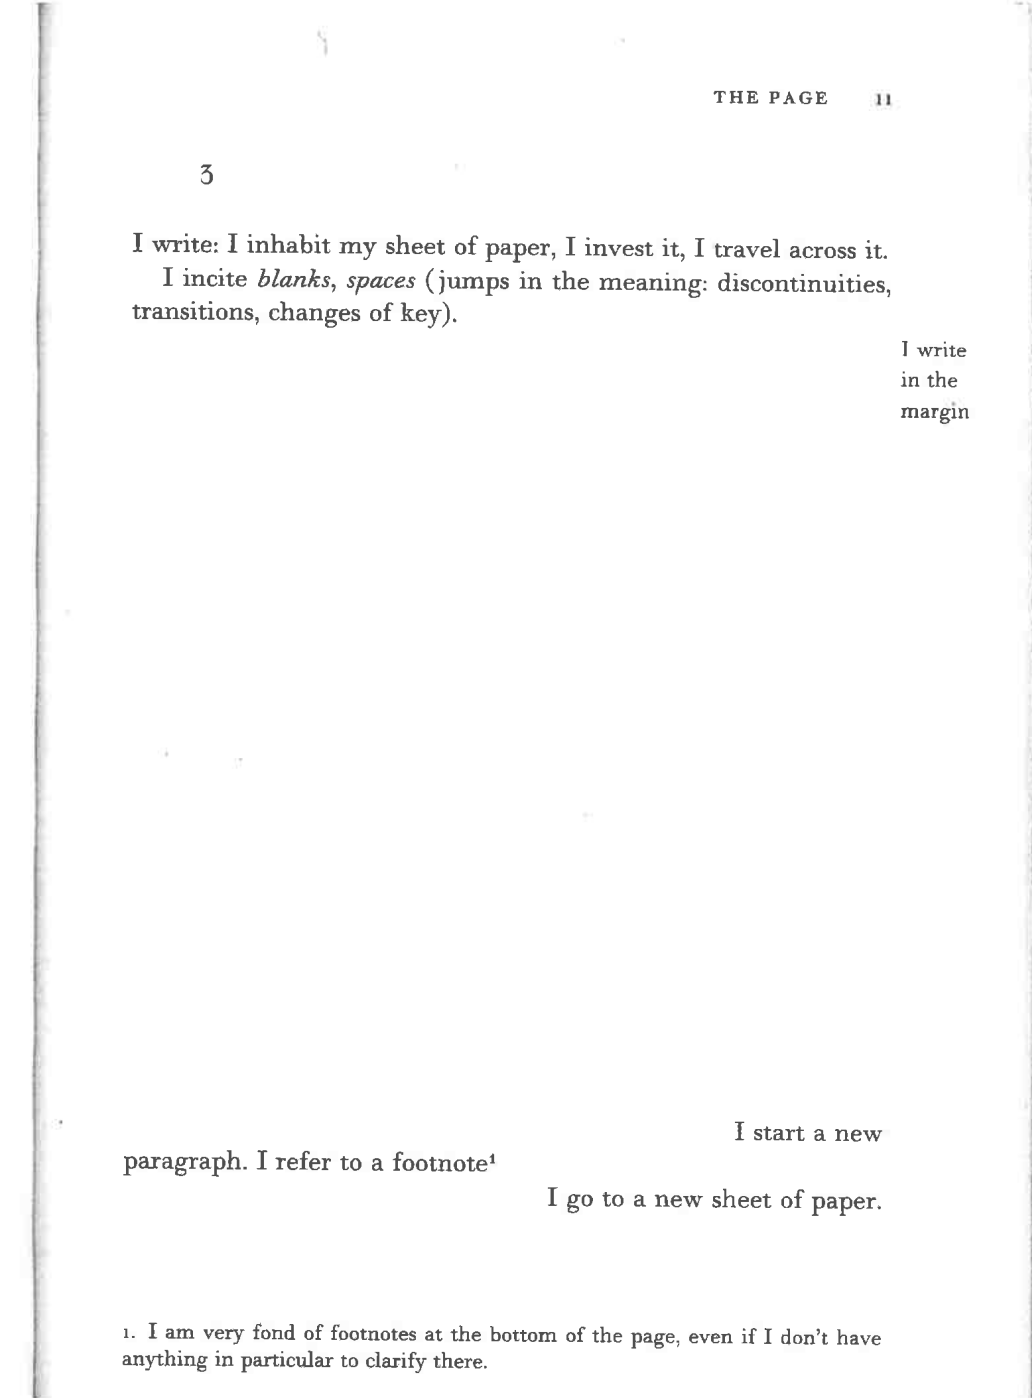
\includegraphics[width=.9\linewidth]{./perec.png}
\end{center} 


\section*{The RC Exposition}
\label{sec:org36e412e}
\begin{itemize}
\item Online rich media format for publication, reviewing, archiving of
artistic research
\item Extended form of academic writing (as making)
\item Reflexivity of aesthetic knowledge
\item Translation of practices
\item Challenging existing practices
\item Answers to everyday problems of the making, dissemination and
publication of artistic research
\end{itemize}

\section*{Challenges}
\label{sec:org5ebfc76}
\begin{itemize}
\item Focus on fixity of publication
\item Note taking and sketching
\item Relating things
\item Absolute positioning (poster and page printing paradigms)
\item "Visucentrism"
\end{itemize}

\section*{The Exposition as a Digital Object}
\label{sec:org740d1ae}
\end{document}